\documentclass[a4paper,12pt]{article}
\usepackage{jheppub} % for details on the use of the package, please see the JINST-author-manual
\usepackage{lineno}
\usepackage{indentfirst}
\usepackage{subcaption} % Add this for subfigure environment
\usepackage{float} % Add this for the [H] float placement option

% \linenumbers



% \arxivnumber{1234.56789} % if you have one

\title{QIC Final Project: Anisotropic Transmission of quantum information through quantum fields}

% Collaborations

%% [A] If main author
%% \collaboration{\includegraphics[height=17mm]{collabroation-logo}\\[6pt]
%%  XXX collaboration}

%% or
%% [B] If "on behalf of"
%% \collaboration[c]{on behalf of XXX collaboration}


% Authors
% The "\note" macro will give a warning: "Ignoring empty anchor...", you can safely ignore it.

%% [A] simple case: 2 authors, same institution
%% \author[1]{A. Uthor\note{Corresponding author.}}
%% \author{and A. Nother Author}
%% \affiliation{Institution,\\Address, Country}

%% or, e.g.
%% [B] more complex case: 4 authors, 3 institutions, 2 footnotes
%% \author[a,b]{F. Irst,\note{Now at another university}}
%% \author[c]{S. Econd,}
%% \author[a,2]{T. Hird\note{Also at Some University.}}
%% \author[c,2]{and Fourth}
%% \affiliation[a]{Institution_1,\\Address, Country}
%% \affiliation[b]{Institution_2,\\Address, Country}
%% \affiliation[c]{Institution_3,\\Address, Country}

\author{T. Hsu}
\affiliation{National Taiwan University,\\
Taipei, Taiwan}
% \affiliation{Another University,\\
% different-address, Country}

% E-mail addresses: only for the corresponding author
\emailAdd{b11901097@ntu.edu.tw}

\abstract{In this letter, we briefly review the possible way to transmit the quantum information via quantum fields \cite{PhysRevD.101.036014}, and then we discuss }



\begin{document}
\maketitle
\flushbottom
% \section{Path Integral in Euclidean Signature}
\section{Quantum Channel: Via Quantum Mechanics}
In quantum information theory, the information is represented by a qubit, and it can be transformed, projected, and transmitted based on basic quantum mechanics posulates.
In this letter, we focus on the transmission of a qubit from a spacetime emitter Alice $ A $ to a receiver Bob $ B $.

There are various ways to transmit a qubit without contacting, which are based on the \textit{resources} Alice and Bob share.
For instance, if an entagled state is shared, they can transmit the qubit by Alice performing the Bell measurement and then send the result (a classical cbit) to Bob, which is the well-known \textit{quantum teleportation}.
Here, we simply consider transmisstion by a third quantum bit $ C $, $ \hat \rho_{ C, 0 } $.
Denote Alice's qubit as $ \hat \rho_{ A, 0 } $ and Bob's qubit $ \hat \rho_{ B, 0 }$; the transmission is done by performing SWAP between $ A $ and $ C $, and then between $ C $ and $ B $. 
The whole process is unitary and does not violate the non-cloning process because Alice's qubit becomes $ \hat \rho_{ C, 0 } $.

The SWAP operator can be derived by assuming $ \hat \rho_{ C, 0 } = | 0 \ar \al 0 |$ and $ \hat \rho_{ A, 0 } = | a \ar \al a | $ with $ \al a | 0 \ar \ne 0 $:
\be
    U \rho_{ A, 0 } \otimes \rho_{ C, 0 } U^{\dagger} = \rho_{ C, 0 } \otimes \rho_{ A, 0 }
\ee


\textbf{Remark: }
The transmission of qubit described above is rather trivial; however, it is based on an important fact that the dimension of the Hilbert space of $ C $ is the same as those of the Hilbert space of $ A $ and $ B $, so there is an isomorphism between the Hilbert spaces.
As we will see in the next section, the Hilbert space (or more precisely, the Fock space) of quantum fields is infinite-dimensional, and therefore there is no isomorphism like SWAP gate in the quantum mechanic case.
\section{Quantum Channel: Via Quantum Fields}
\subsection{Brief Review on Quantum Field Theory}
\subsection{Unruh-DeWitt model}

\section{Non-isotropic Smearing Function}
\subsection{Problem Setup}
The smearing function used in the paper is isotropic (i.e., $F_A = \frac{1}{\sqrt{\pi}\sigma} \exp\left(-\frac{|\mathbf{x}|^2}{\sigma^2}\right)$), which leads to isotropic propagation of information. In our study, we aim to investigate whether employing a non-isotropic smearing function could lead to different behavior.

As a first step, we consider a smearing function $F_A$ with axial symmetry, i.e., $F_A = R(r)\Theta(\theta)$.
And do fallowing simplification, 
\begin{enumerate}
  \item $R(r)$ is localized at $r = 0$, i.e., $R(r \rightarrow \infty) = 0$
  \item $\Theta(\theta) = \frac{\delta(\theta)}{\sin{\theta}}$,
\end{enumerate}
where the $\frac{1}{\sin\theta}$ factor arises from the solid angle element in spherical coordinates.
The reason of first simplification is that Alice should not able to encode the information with the infinite range. And the reason of second simplification is the delta function should provide a well non-isotropic condition.

Under this construction, the smearing function $F_{B1}$ becomes
\be
    F_{B1}(\mathbf{x}) = - \int \mathrm{d}r\, \mathrm{d}\theta\, \mathrm{d}\phi\, r^2 \sin{\theta} \, R(r)\frac{\delta(\theta)}{\sin{\theta}} \frac{\delta\left(\left|\mathbf{r} - \mathbf{x}\right| - \Delta\right)}{4\pi\left|\mathbf{r} - \mathbf{x}\right|}
\ee
To evaluate the delta function, we use the following identity:
\[
    \int \mathrm{d}x g(x) \delta(f(x)) = \int \mathrm{d}f \frac{g}{\left|f'\right|} \delta(f) = \sum_i\frac{g(x_i0)}{\left|f'(x_{i0})\right|}
\]
where $x_{i0}$ are all $x$ within the domain of integration which satisfy $f(x_{i0}) = 0$. Since in our case, we only integrate over positive real values of $r$, we only consider the solutions $r \in \mathbb{R}^+$ in the following calculation.

Before proceeding, we need to express $|\mathbf{r} - \mathbf{x}|$ in terms of $(r, \theta, \phi)$, so that we can perform the integration explicitly. Given that the smearing function is axially symmetric, we align $\mathbf{x}$ along the $\phi = 0$ plane, i.e., we choose coordinates such that $\mathbf{x} = (x, \theta_x, 0)$, since any $\mathbf{x} = (x, \theta_x, \phi)$ yields the same value due to the symmetry. Then, the distance between $\mathbf{r}$ and $\mathbf{x}$ can be written as
\[
|\mathbf{r} - \mathbf{x}| = \sqrt{r^2 + x^2 - 2rx \cos\gamma},
\]
where $\gamma$ is the angle between $\mathbf{r}$ and $\mathbf{x}$. Using the spherical coordinate expression for the angle between two vectors, we have
\[
\cos\gamma = \cos\theta \cos\theta_x + \sin\theta \sin\theta_x \cos\phi.
\]
The whole function becomes
\be
    F_{B1}(\mathbf{x}) = - \int \mathrm{d}\theta\, \mathrm{d}\phi\, \mathrm{d}r\, r^2 \, R(r) \delta(\theta) \frac{\delta\left(\sqrt{r^2 + x^2 - 2rx \cos\gamma} - \Delta\right)}{4\pi\sqrt{r^2 + x^2 - 2rx \cos\gamma}}
\ee
The solutions of $\sqrt{r^2 + x^2 - 2rx \cos\gamma} - \Delta = 0$ are
\[
    r_\pm = x\cos\gamma \pm \sqrt{x^2 \cos^2\gamma - (x^2 - \Delta^2)}
\]
We mention before, we only need the positive real solutions. So now we discuss when will $r_\pm$ be positive, when will be negative, or even be complex.
\begin{center}
  \begin{tabular}{|c|c|c|c|c|}
    \hline
    $\cos{\gamma} > 0$ & $\Delta^2 > x^2$ & $\left|\sin\gamma\right| < \frac{\Delta}{x}$ & remain solutions & reason of unavalible\\
    \hline\hline
    True & True & - & + & $\mathbb{R^-}$\\
    True & False & True & $\pm$ & -\\
    True & False & False & 0 & $\mathbb{C-R}$\\
    False & True & - & + & $\mathbb{R^-}$\\
    False & False & - & 0 & $\mathbb{R^-}$\\
    \hline
  \end{tabular}
\end{center}
Then we do another simplification, that is setting $\theta_x = 0, \pi$, i.e., align $\mathbf{x}$ on the axis of $\mathbf{r}$. The reason we do this simplification is that we wonder how should Bob measure the field on the axis where also should has the most significant non-isotropic phenonenon.
\subsection{Result}
Since we set $\theta_x = 0, \pi$ and the delta function makes the smearing function only distribute in $\theta = 0$, we can rewrite $\cos\gamma$ as $1, -1$, and $r_\pm$ as $x \pm \Delta, - x \pm \Delta$. We now able to derive the $F_{B1}$ explicitly.
\begin{align}
    F_{B1}(\mathbf{x}) &= - \int \mathrm{d}\theta\, \delta(\theta)  \int \mathrm{d}\phi\, \int \mathrm{d}r\, r^2 \, R(r) \frac{\delta\left(\sqrt{r^2 + x^2 - 2rx \cos\gamma} - \Delta\right)}{4\pi \sqrt{r^2 + x^2 - 2rx \cos\gamma}} \notag \\
                       &= - \frac{1}{2} \sum \frac{r_{\pm}^2 R(r_{\pm})}{\sqrt{r_{\pm}^2 + x^2 - 2r_{\pm}x\cos\gamma}} \frac{1}{\frac{r_{\pm} - x\cos\gamma}{\sqrt{r_{\pm}^2 + x^2 - 2r_{\pm}x\cos\gamma}}} \notag \\
                       &= 
                       \begin{cases}
                           - \frac{1}{2} \sum \frac{r_{\pm}^2}{r_{\pm} - x} R(r_{\pm}) & \text{if } \theta_x = 0 \\
                           - \frac{1}{2} \sum \frac{r_{\pm}^2}{r_{\pm} + x} R(r_{\pm}) & \text{if } \theta_x = \pi \\
                       \end{cases} \notag \\
                       &=
                       \begin{cases}
                           - \frac{1}{2} \frac{(x + \Delta)^2}{(x + \Delta) - x} R(x + \Delta) & \text{if } \theta_x = 0 \wedge \Delta^2 > x^2 \\
                           - \frac{1}{2} \left(\frac{(x + \Delta)^2}{(x + \Delta) - x} R(x + \Delta) + \frac{(x - \Delta)^2}{(x - \Delta) - x} R(x - \Delta)\right) & \text{if } \theta_x = 0 \wedge \Delta^2 < x^2 \\
                           - \frac{1}{2} \frac{(\Delta - x)^2}{(\Delta - x) + x} R((\Delta - x)) & \text{if } \theta_x = \pi \wedge \Delta^2 > x^2 \\
                           0 & \text{if } \theta_x = \pi \wedge \Delta^2 < x^2 \\
                       \end{cases} \notag \\
                       &=
                       \begin{cases}
                           - \frac{1}{2\Delta} (x + \Delta)^2 R(x + \Delta) & \text{if } \theta_x = 0 \wedge \Delta^2 > x^2 \\
                           - \frac{1}{2\Delta} \left((x + \Delta)^2 R(x + \Delta) - (x - \Delta)^2 R(x - \Delta)\right) & \text{if } \theta_x = 0 \wedge \Delta^2 < x^2 \\
                           - \frac{1}{2\Delta} (\Delta - x)^2 R((\Delta - x)) & \text{if } \theta_x = \pi \wedge \Delta^2 > x^2 \\
                           0 & \text{if } \theta_x = \pi \wedge \Delta^2 < x^2 \\
                       \end{cases} \notag \\
\end{align}
Note that when \( \theta_x = \pi \), the smearing function of Bob is located directly behind that of Alice along the same axis. Therefore, if we are only interested in the behavior of the smearing function along this axis, we can equivalently set \( x \rightarrow -x \) while taking \( \theta_x = \pi \). So the smearing function becames
\be
    F_{B1}(\mathbf{x}) =
                       \begin{cases}
                           - \frac{1}{2\Delta} \left((x + \Delta)^2 R(x + \Delta) - (x - \Delta)^2 R(x - \Delta)\right) & \text{if } \Delta < x \\
                           - \frac{1}{2\Delta} (x + \Delta)^2 R(x + \Delta) & \text{if } -\Delta < x < \Delta \\
                           0 & \text{if } x < -\Delta \\
                       \end{cases} \notag \\
\ee
We can try to plug in the Gaussian function to $R(r)$ first. And get fallowing figure,
\begin{figure}[H]
    \centering
    \begin{subfigure}[b]{0.45\textwidth}
         \centering
         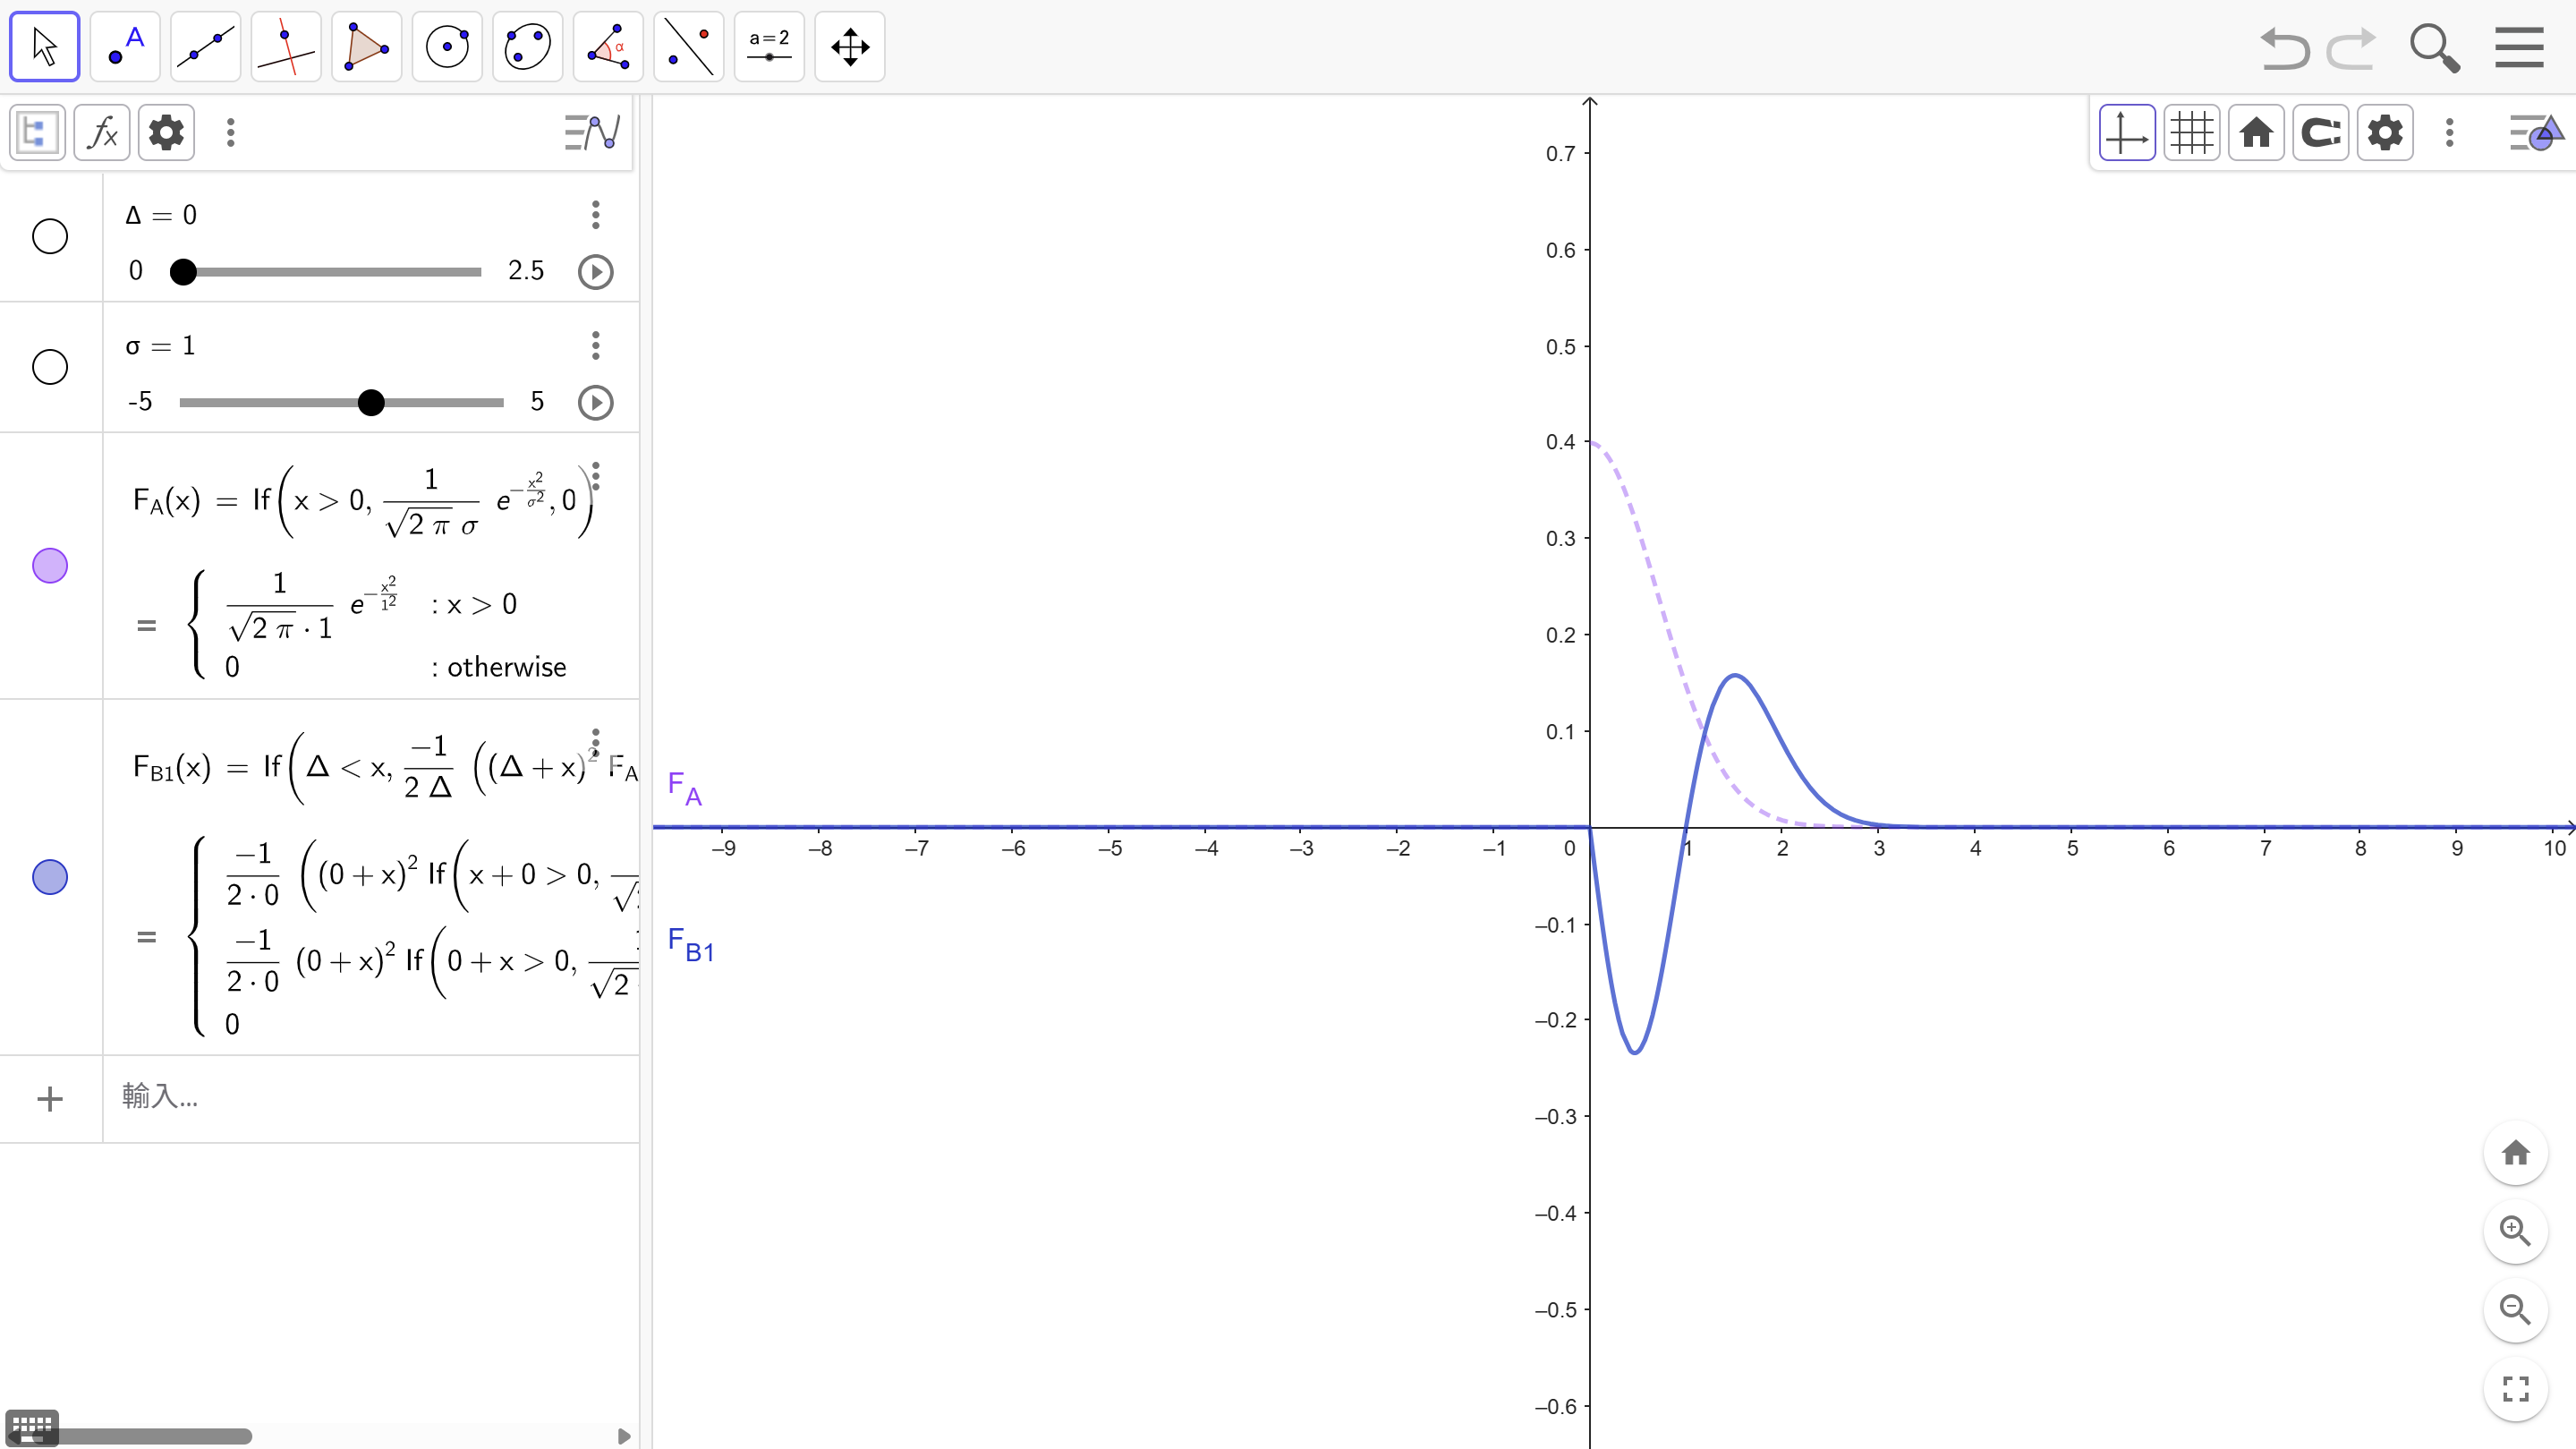
\includegraphics[width=\textwidth]{fig/Fa0.png}
         \caption{t $\rightarrow$ 0}
         \label{fig:t0}
    \end{subfigure}
    \hfill
    \begin{subfigure}[b]{0.45\textwidth}
         \centering
         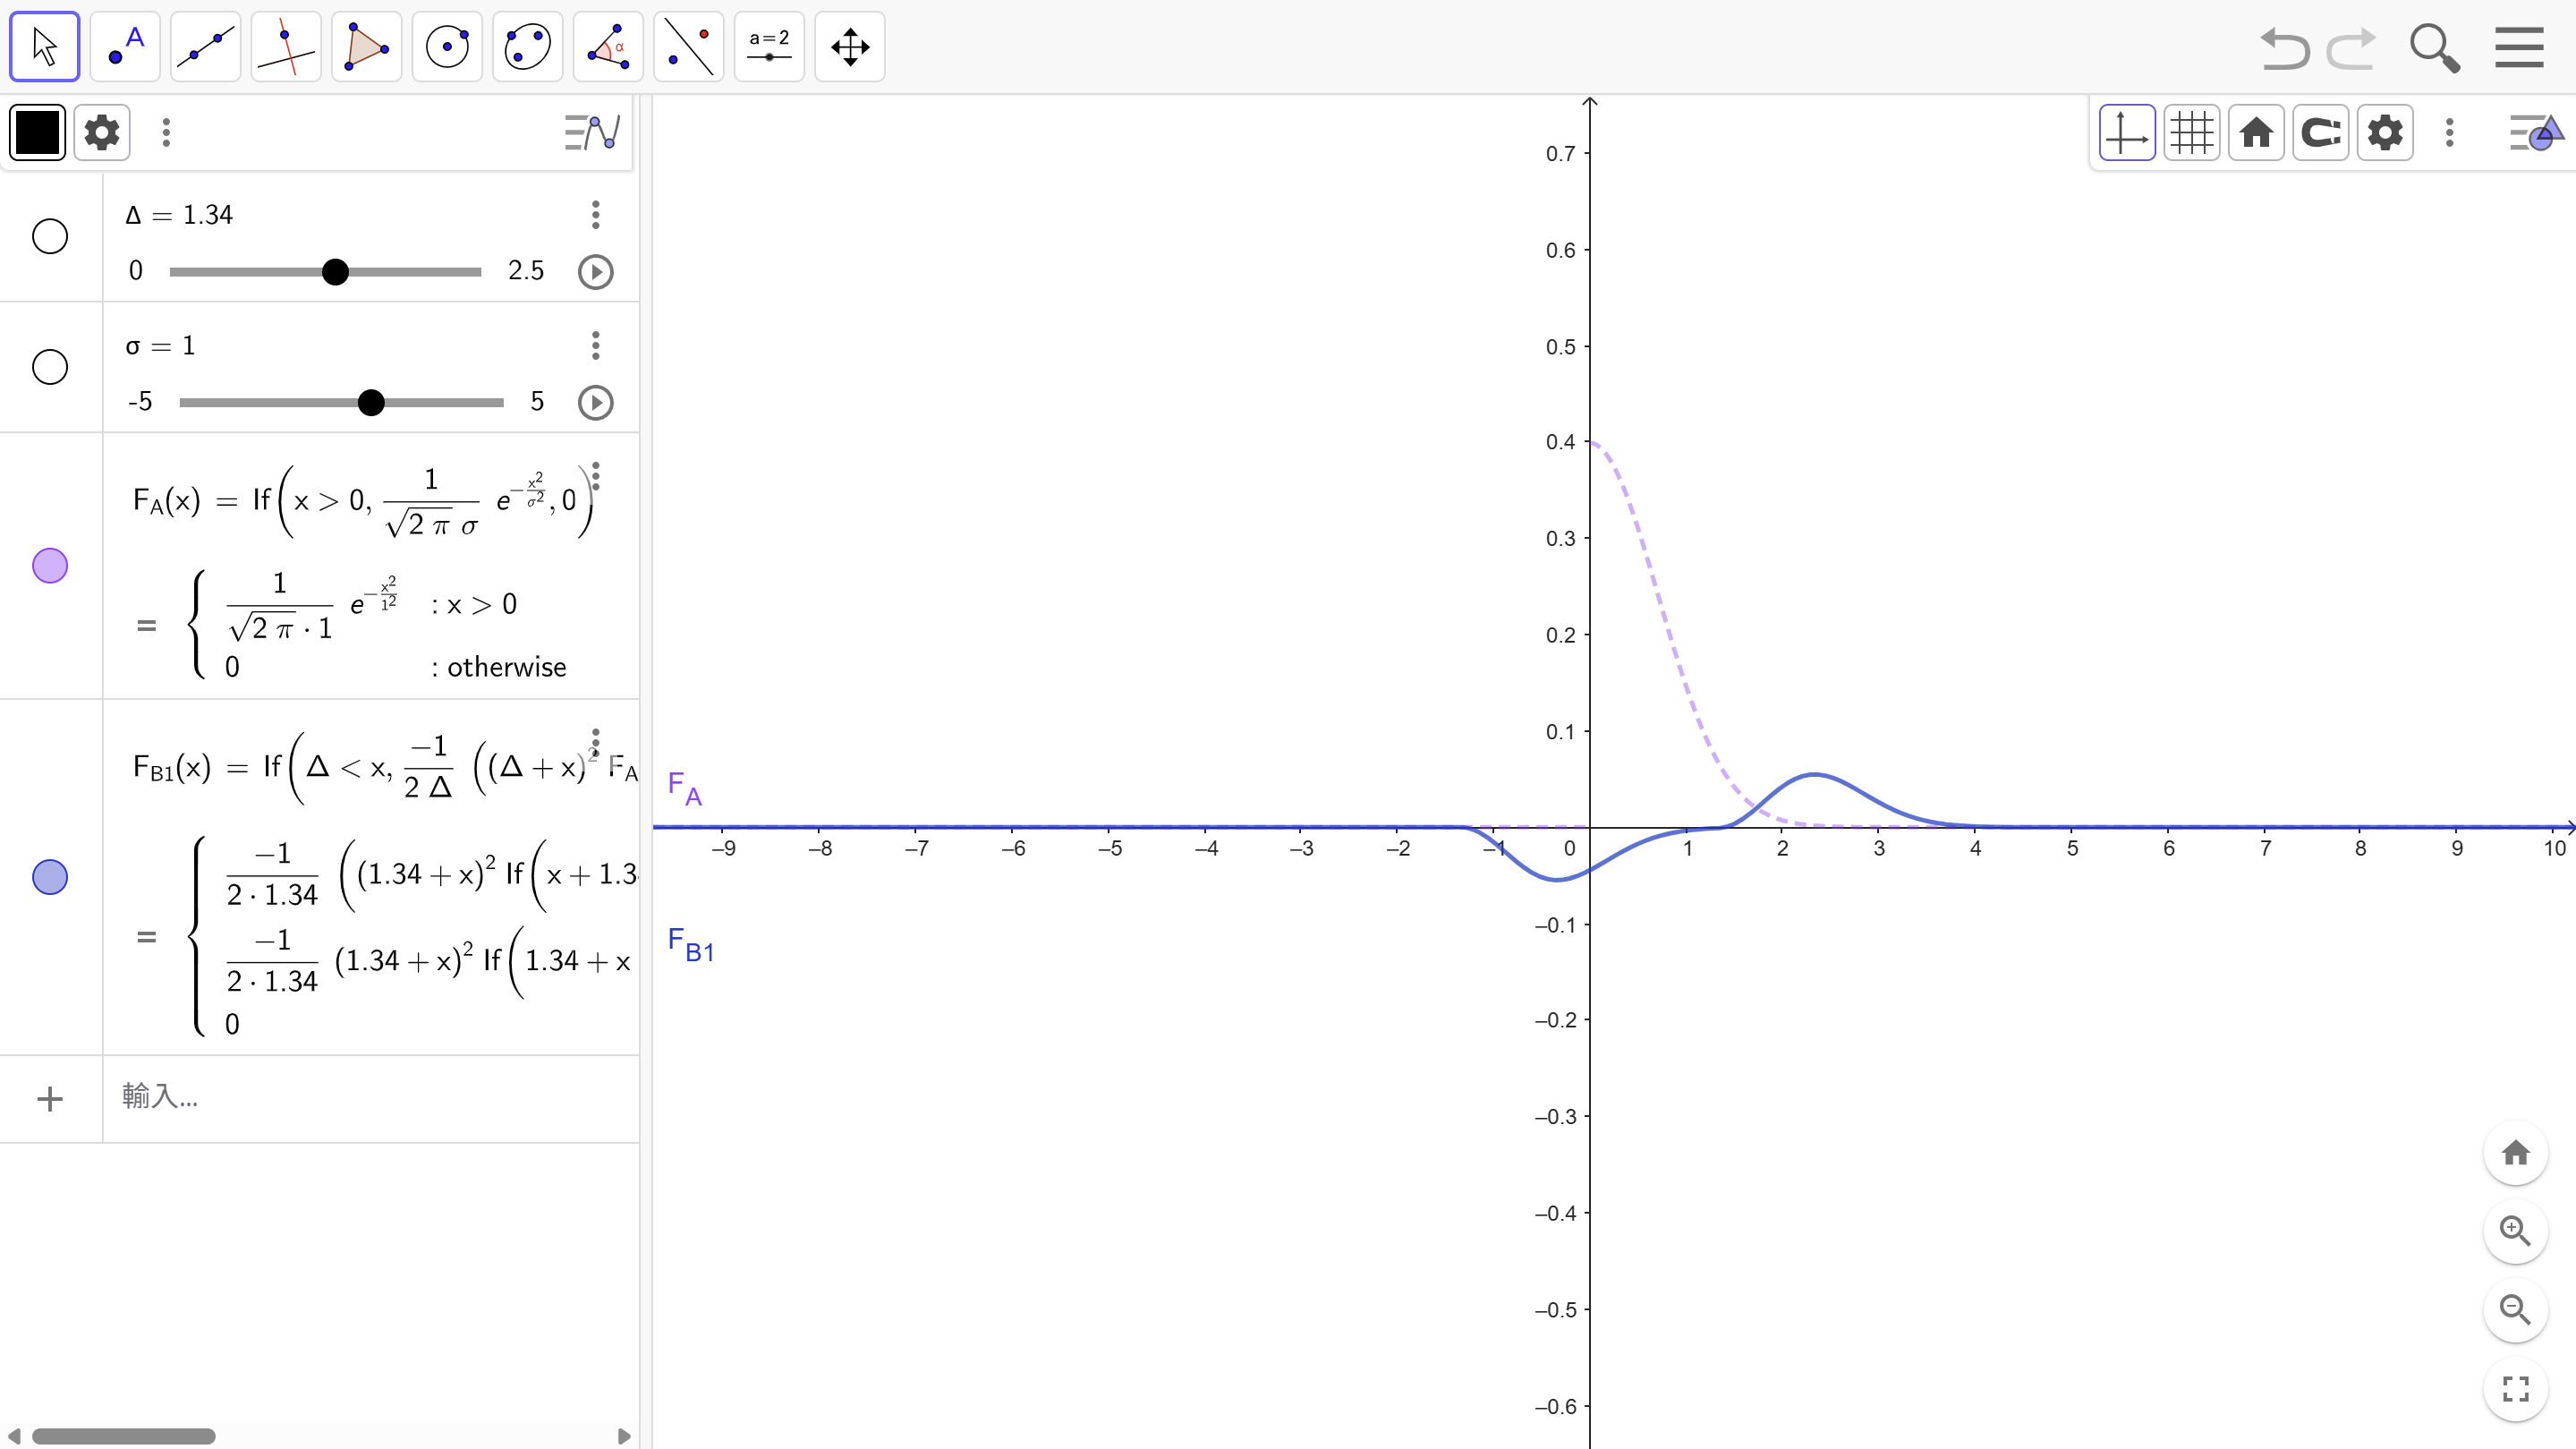
\includegraphics[width=\textwidth]{fig/Fa1.png}
         \caption{t = 1.34}
         \label{fig:t1}
    \end{subfigure}
    \hfill
    \begin{subfigure}[b]{0.6\textwidth}
         \centering
         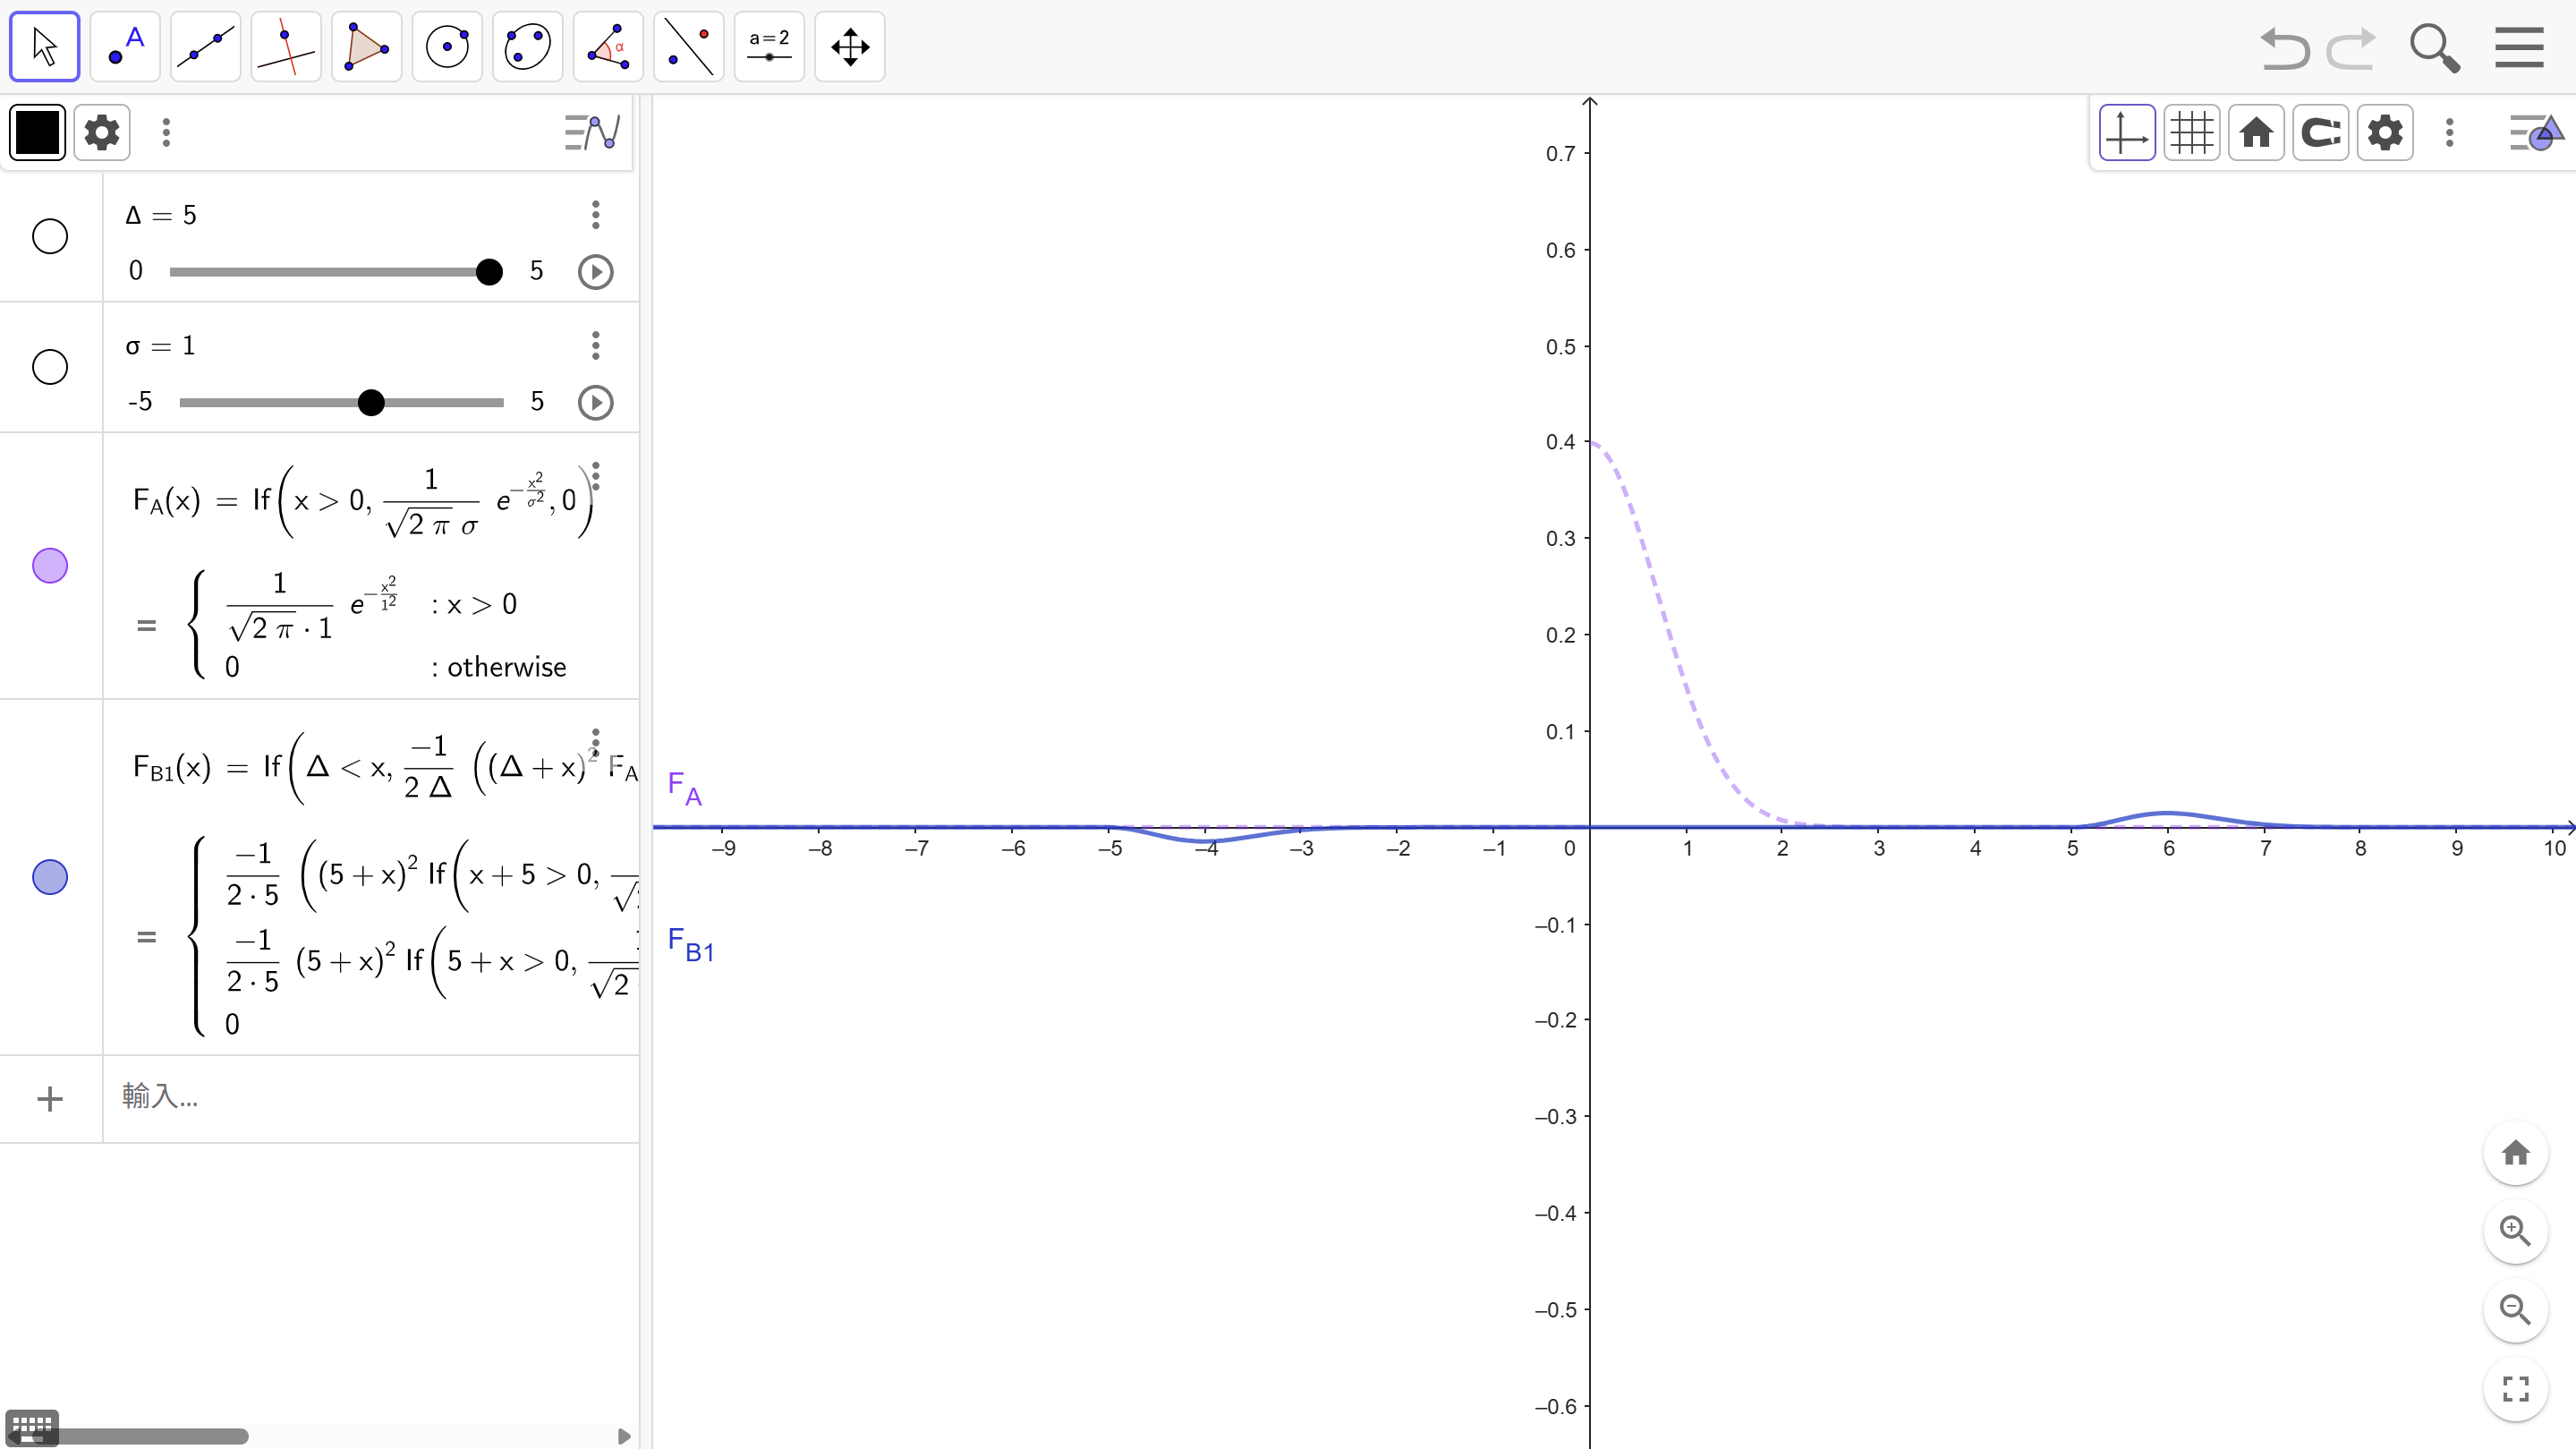
\includegraphics[width=\textwidth]{fig/Fa2.png}
         \caption{t = 5}
         \label{fig:t2}
    \end{subfigure}
\end{figure}
From the figures above, we can observe that the propagation of $F_{B1}$ does not exhibit any non-isotropic behavior. The distribution remains symmetric along the axis, indicating that the chosen smearing function, despite being non-isotropic, does not lead to anisotropic propagation in this setup.

It is similar to calculate \(F_{B2}, F_{B3}\), we could explicitly write out what they are, 
\begin{equation}
    F_{B2}(\mathbf{x}) = - \int \mathrm{d}\theta\, \delta(\theta)  \int \mathrm{d}\phi\, \int \mathrm{d}r\, r^2 \, R(r) \frac{\delta '\left(\sqrt{r^2 + x^2 - 2rx \cos\gamma} - \Delta\right)}{4\pi \sqrt{r^2 + x^2 - 2rx \cos\gamma}} \notag \\
\end{equation}
\begin{equation}
    F_{B3}(\mathbf{x}) = - \int \mathrm{d}\theta\, \delta(\theta)  \int \mathrm{d}\phi\, \int \mathrm{d}r\, r^2 \, R(r) \frac{\delta ''\left(\sqrt{r^2 + x^2 - 2rx \cos\gamma} - \Delta\right)}{4\pi \sqrt{r^2 + x^2 - 2rx \cos\gamma}} \notag \\
\end{equation}
where \(\displaystyle \delta '(x) = \frac{d \delta(x)}{d x}\) and \(\displaystyle \delta '''(x) = \frac{d^2 \delta(x)}{d x^2}\). Note that is derivative is differential over x, in the original equation, it becomes differentialing over \(\sqrt{r^2 + x^2 - 2rx \cos{\gamma}}\). Thus we need to do a change of variable, Chain rule, to change the variable to \(r\). After these messy calculation, we obtain the following equations
\begin{equation}
    F_{B2}(\mathbf{x}) = \int \frac{1}{\Delta}\left(\delta '(r - r_+) + \delta '(r - r_-) \right)g(r) r^2 R(r) \mathrm{d} r 
\end{equation}
\begin{equation}
    F_{B3}(\mathbf{x}) = \int \frac{1}{\Delta}\left(g(r) (\delta '(r - r_+) + \delta '(r - r_-)) \right) g(r) r^2 R(r) \mathrm{d} r 
\end{equation}
where \(g(r) = \frac{d r}{d \sqrt{r^2 + x^2 - 2rx \cos{\gamma}}}\).
By using the following properties of Dirac delta function,
\begin{align}
    &\int \mathrm{d} x \, \delta '(x-a) f(x) = f'(a)\\
    &\int \mathrm{d} x \, \delta ''(x-a) f(x) = f''(a)
\end{align}
we obtain 
\begin{align*}
    F_{B2}(\mathbf{x}) &= \frac{\Delta  (\Delta -x) e^{-\frac{(x-\Delta )^2}{\sigma ^2}} \left((x-\Delta )^2-\sigma ^2\right)}{\sqrt{\Delta ^2} \sigma ^2}\operatorname{sgn}(x - \Delta)\\ &+\frac{\Delta  (\Delta +x) e^{-\frac{(\Delta +x)^2}{\sigma ^2}} \left((\Delta +x)^2-\sigma ^2\right)}{\sqrt{\Delta ^2} \sigma ^2} \operatorname{sgn}(x + \Delta)
\end{align*}

{\footnotesize\begin{align*}
    F_{B3}(\mathbf{x}) &= \frac{e^{-\frac{(x-\Delta )^2}{\sigma ^2}} \left(-5 \Delta ^2 \sigma ^2+2 \Delta ^4+\sigma ^4+x^2 \left(12 \Delta ^2-5 \sigma ^2\right)-8 \Delta  x^3+2 x^4+x \left(10 \Delta  \sigma ^2-8 \Delta ^3\right)\right)}{\sigma ^4}\operatorname{sgn}(x - \Delta)\\
    &+\frac{e^{-\frac{(\Delta +x)^2}{\sigma ^2}} \left(-5 \Delta ^2 \sigma ^2+2 \Delta ^4+\sigma ^4+x^2 \left(12 \Delta ^2-5 \sigma ^2\right)+8 \Delta  x^3+2 x^4+2 x \left(4 \Delta ^3-5 \Delta  \sigma ^2\right)\right)}{\sigma ^4}\operatorname{sgn}(x + \Delta) 
\end{align*}}
The figure of both is plotted below, we can see that it is indeed surviving in the \(\theta = 0\) direction and \(\theta = \pi\) direction. Thus we can't make a isotropic quantum teleportation via this setup.

% \begin{figure}[htbp]
%     \centering
%     \subfigure[FB2]{
%         \includegraphics[width=0.45\textwidth]{FB2.pdf}
%         \label{fig:sub1}
%     }
%     \hfill
%     \subfigure[FB3]{
%         \includegraphics[width=0.45\textwidth]{FB3.pdf}
%         \label{fig:sub2}
%     }
%     \caption{Comparison of FB2 and FB3}
%     \label{fig:combined}
% \end{figure}

\appendix

\acknowledgments

% Bibliography

%% [A] Recommended: using JHEP.bst file
%% \bibliographystyle{JHEP}
%% \bibliography{biblio.bib}

%% or
%% [B] Manual formatting (see below)
%% (i) We suggest to always provide author, title and journal data or doi:
%% in short all the informations that clearly identify a document.
%% (ii) please avoid comments such as "For a review'', "For some examples",
%% "and references therein" or move them in the text. In general, please leave only references in the bibliography and move all
%% accessory text in footnotes.
%% (iii) Also, please have only one work for each \bibitem.
\bibliographystyle{plain}
\bibliography{ref}

% Example reference entry in ref.bib
% @article{example_reference,
%   author = {Author Name},
%   title = {Example Title},
%   journal = {Example Journal},
%   year = {2023},
%   volume = {1},
%   pages = {1--10}
% }
\end{document}
